\section{Implementation}

\subsection{Supporting tools}

\subsubsection{Track Splicer}
This project is designed to work with any race track given specific track meta data is provided to aid the feedback system processing. The meta data is split into two files, the first is the race line file which contains data from which the feedback system can determine the race line a user should stick to. 
 For this particular study the race line files have been generated from an .ai file which is supplied with Assetto Corsa. Each track has an associated 'ideal\_line.ai' file associated with it. The ai file contains raw bytes, which through manual investigation of the file in hex view, it was noted the file is made of a header part of 36 bytes, followed by a sequence of repeating records of 20 bytes each. These records contain four floats and one 32bit integer, storing the data which is required in the ‘raceline.csv’ file. The records in the ai file are read via a custom developed command line tool and translated into the csv format required by the feedback system. 	

Moving on to the ‘sections.csv’, this file is also a coma separated file containing a sequence of records. These records denote corners and straights which make up the track, and will be used to compute any feedback which is specific to straights or corners. In order to generate this file a tool has been developed which loads the ‘raceline.csv’ and computes the rate of change from one data point to the next. Depending on the rate of change the points are classified as either part of a straight section or as a corner section. This is done by taking three points, p1, p2 and p3 from which two vectors are generated v1 and v2. V1 is the vector from p1 to p2, and v2 is the vector from p2 to p3. Then, v1 and v2 are normalised and the dot product computed which give out the rate of change in radians. The pseudo code for this is shown below.\\

for (i = 0; i < racelinePoints.Count - 2; i++)\\
\{\\
Vector2 v1 = racelinePoints[i].GetVectorToPoint(racelinePoints[i+1]);\\
Vector2 v2 = racelinePoints[i+1].GetVectorToPoint(racelinePoints[i+2]);\\
V1 = Vector2.Normalize(v1);\\
V2 = Vector2.Normalize(v2);\\
float dotProduct = Vector2.Dot(v1, v2);\\
double difference = Math.Acos(dotProduct);\\
\}\\

The corner mid-point can be defined as the highest section of the arch. In order to find this, it is simply a matter of finding the highest possible vector dot product from the section starting point, to the end of the section. The pseudo code is shown below.\\

Point p = endPoint - startPoint;\\
Vector2 n = new Vector2(-p.Y, p.X);\\
Int idOfMax = -1;\\
float max = -1;\\
for (i = trackSection.StartPoint; i <= trackSection.EndPoint; i++)\\
\{\\
p = \_RacingLine[i] - startPoint;\\
float result = Vector2.Dot(new Vector2(point.X, point.Y), n);\\
result = Math.Abs(result);\\
if (result > max)\\
\\{\\
	max = result;
	idOfMax = i;
	\\}\\
\}

\ref{fig:TrackSplicerTool} shows the tool in action which also provides a visual representation of the race line. Corner sections are shows are show are red dots, with green dots used to highlight a corner’s mid-point and straights are shown in blue.

\begin{figure}[!htb]
	\centering
	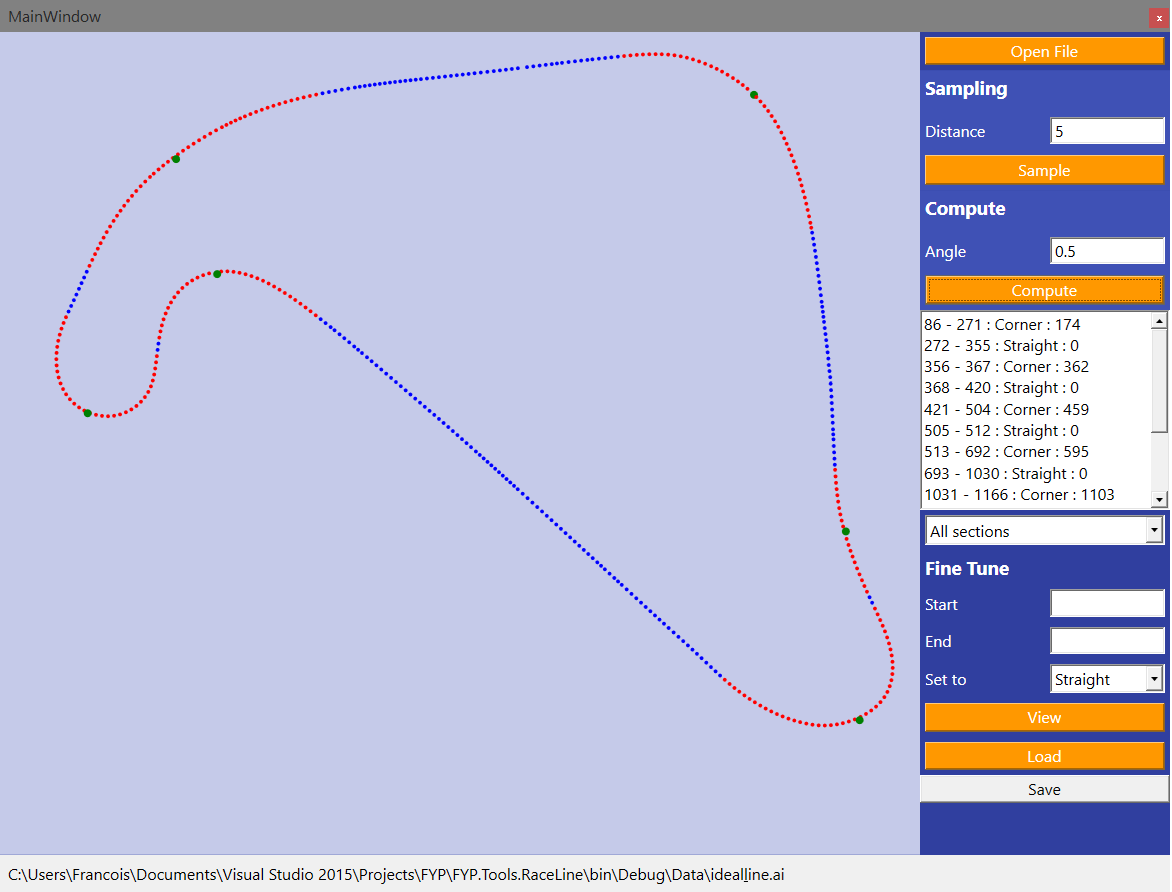
\includegraphics[height=7cm]{images/tracksplicertool}
	\caption{Track splicer tool}
	\label{fig:TrackSplicerTool}
\end{figure}

\subsubsection{Spatial Querying}
As previously mentioned it is important for the feedback system to be able to carry out fast spatial querying operations. A query for the nearest race line data point based relative to the current position of the car is required to be carried out multiple times per second. Thanks to the implementation of a quad tree, the search guaranteed to take place in O(logn), while insertion is done O(nlogn) however, this is not too relevant as all insertion are carried out before the feedback system starts its computations. This structure allows the feedback to quickly calculate in which section of the track the car is located, the nearest race line data point and how far from the race line the car is.

\begin{figure}[!htb]
	\centering
	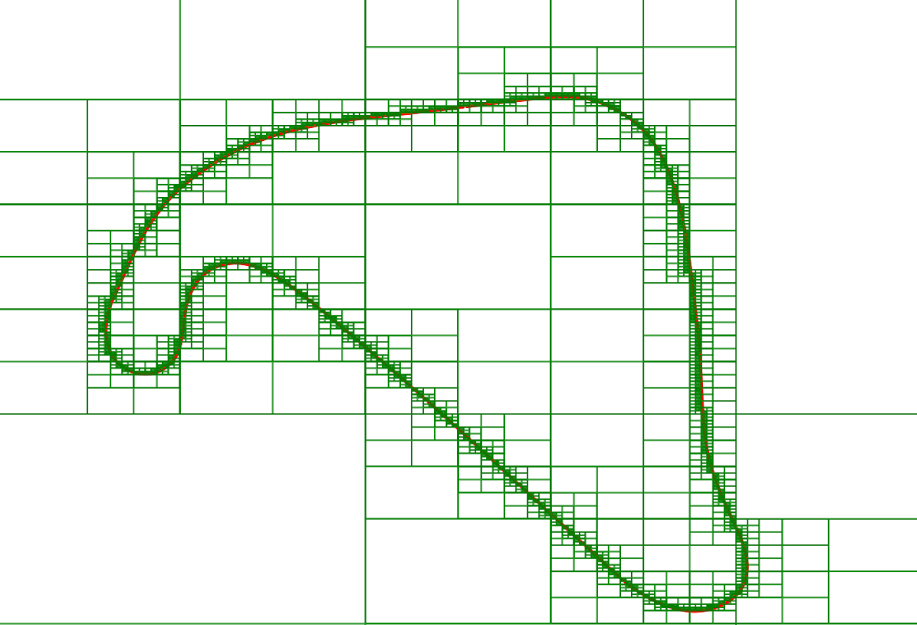
\includegraphics[height=7cm]{images/QuadTree}
	\caption{Visual representation for part of the quad tree}
	\label{fig:QuadTree}
\end{figure}

\subsection{System Architecture}

\begin{figure}[!htb]
	\centering
	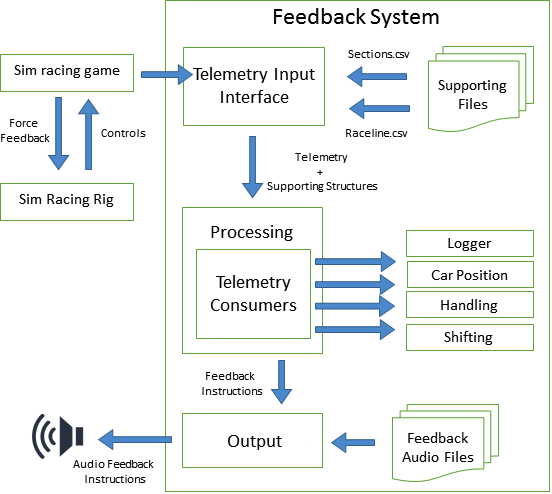
\includegraphics[height=14cm]{images/SystemArch}
	\caption{Overview of the system architecture components}
	\label{fig:SystemArch}
\end{figure}

\subsubsection{Sim Racing Rig}
The rig is made out of various independent components. The steering wheel is a G25 purpose built by Logitech, an electronic steering wheel designed for sim racing video games. It has a 900 degree range of rotation, two force feedback motor and comes as package which includes a pedal set and an H shifter. The pedal set is made of three pedals, from left to right, a clutch pedal, brake pedal and an accelerate pedal. The H shifter simulates one which is found cars fitted with a manual gearbox, the shifter simulates six gears and one reverse. The steering wheel, pedals and shifter are mounted on a home made metal frame which mimics the position of these components as they would be placed in a race car. The last component of the rig is the seat, which is a bucket racing seat which has been taken of a real race car and fitted to racing rig.

\begin{figure}[!htb]
	\centering
	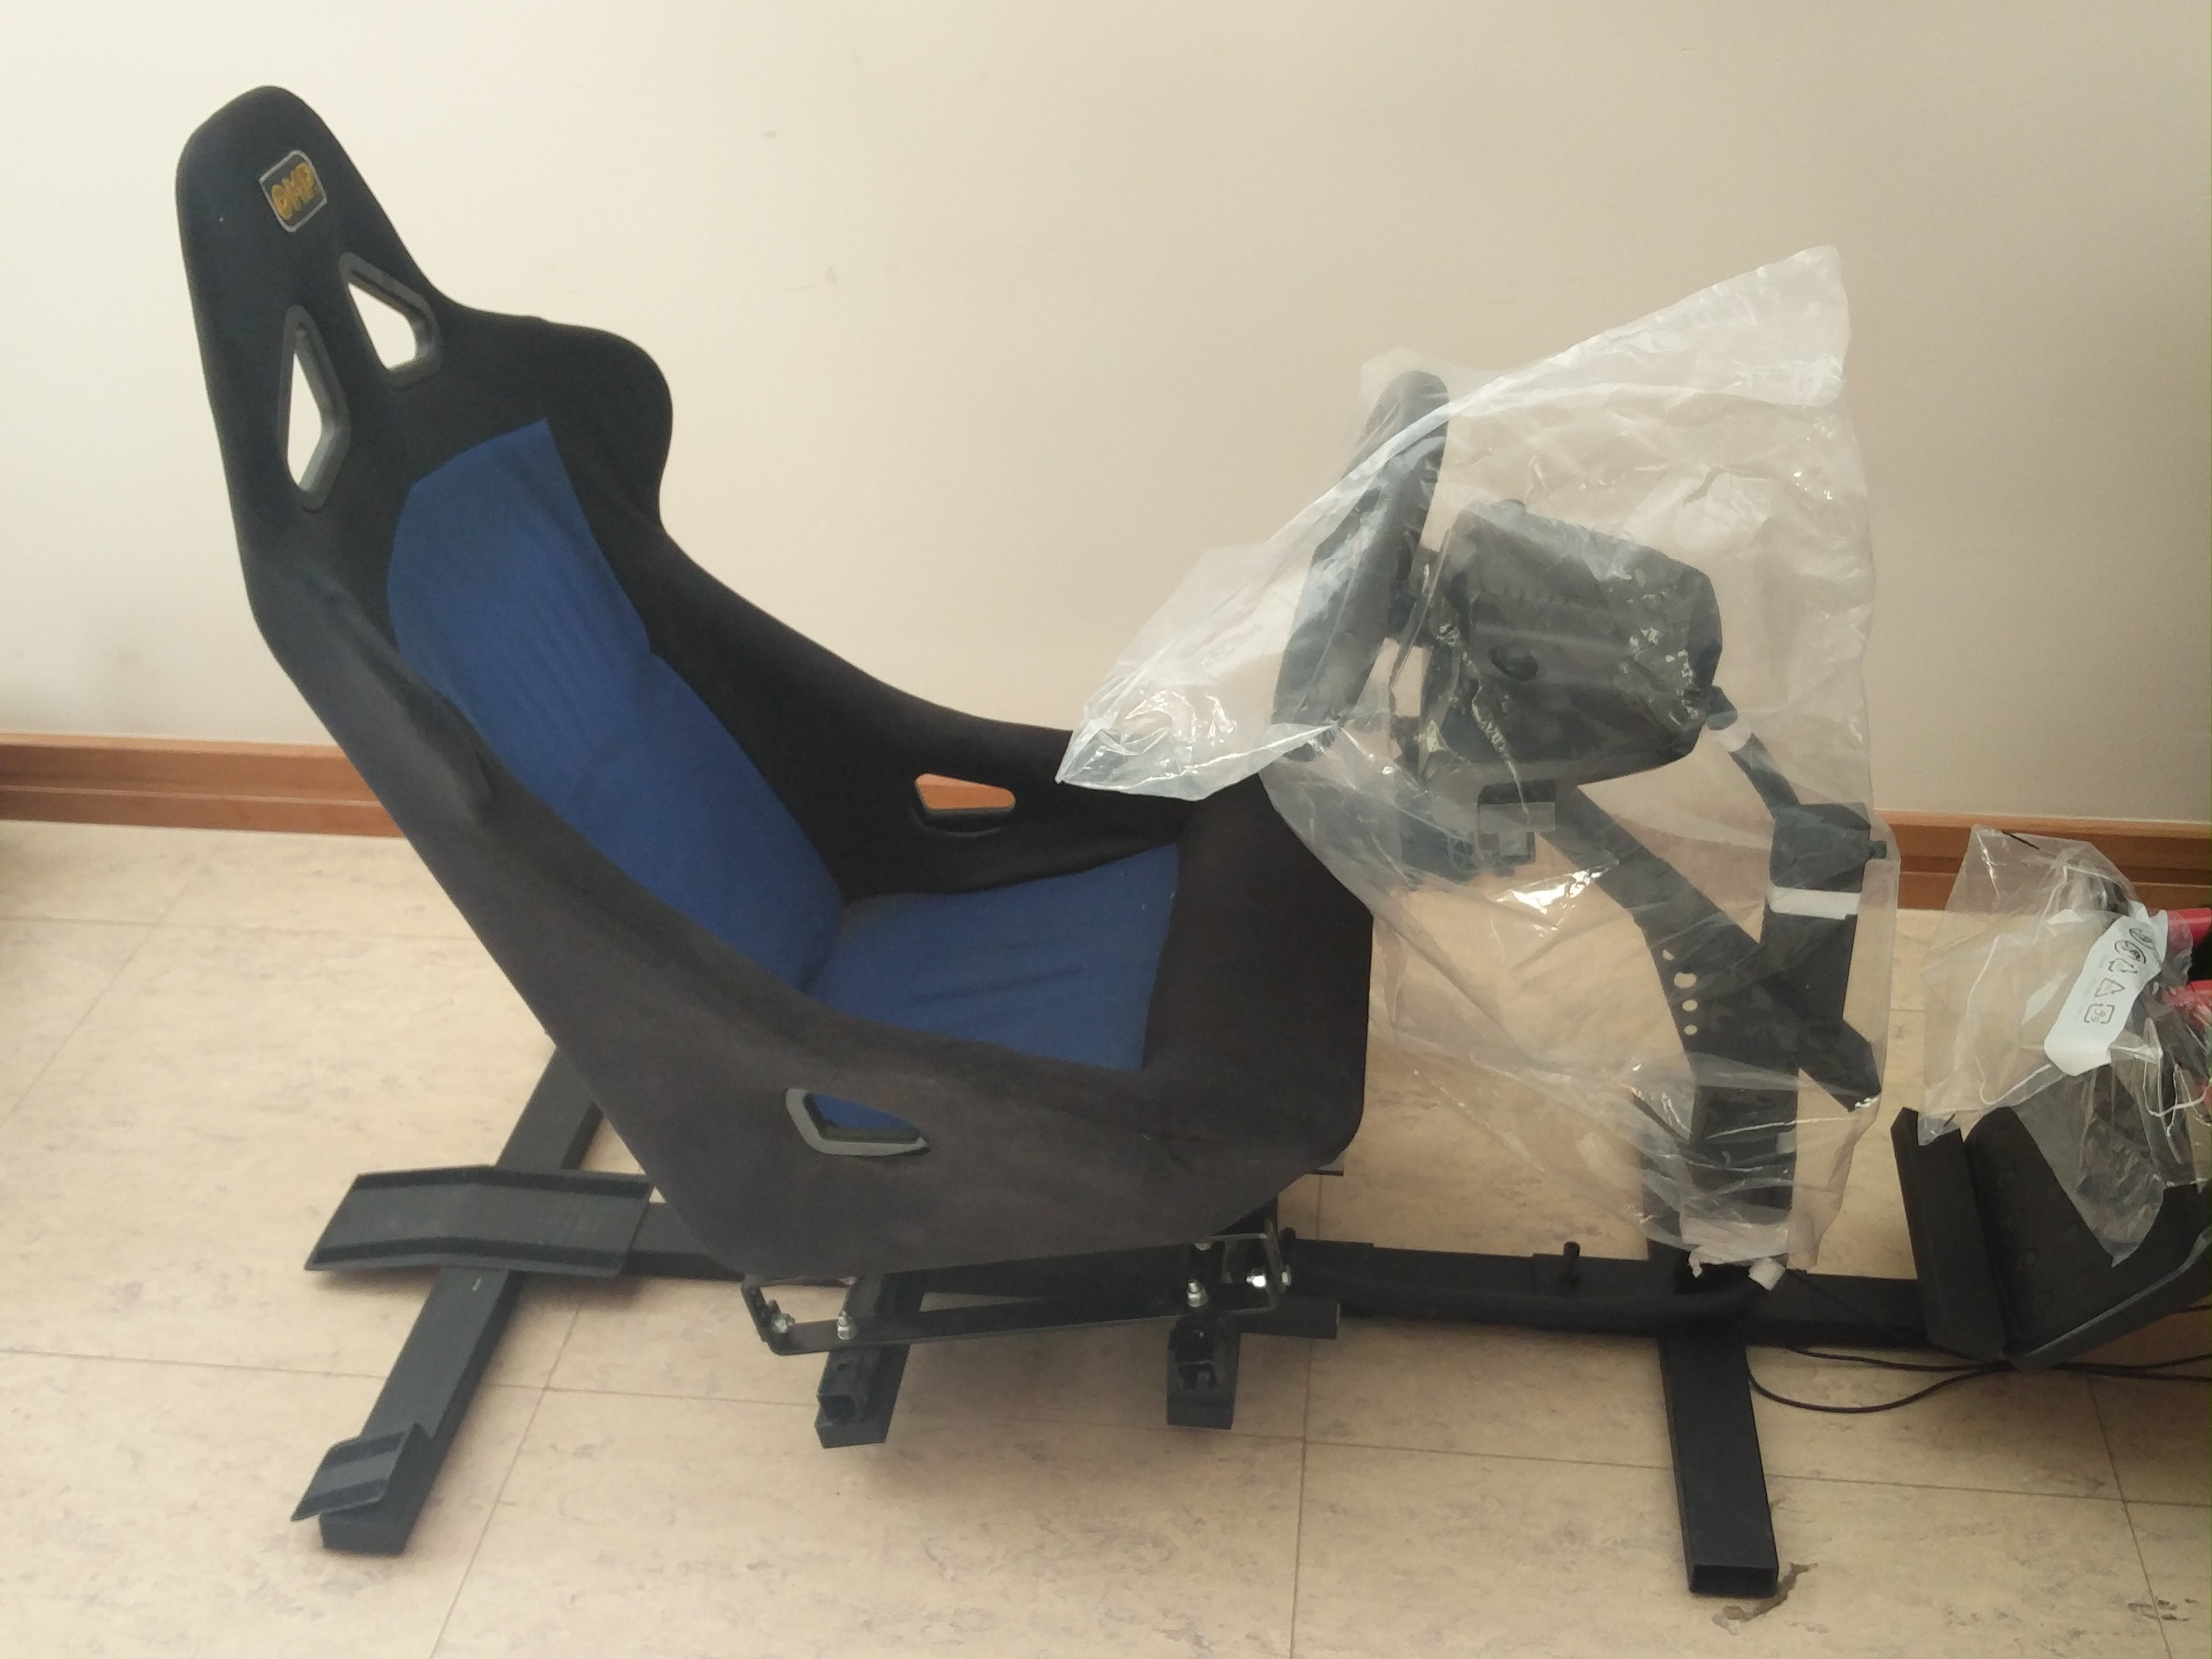
\includegraphics[height=10cm]{images/RacingRig}
	\caption{Side view of the racing rig}
	\label{fig:RacingRig}
\end{figure}

\subsubsection{Feedback system}
Software development of the feedback system has been achieved using C\# and Microsoft's .Net framework. The feedback system is made up of smaller components which pass data to each other in order to produce the feedback instruction which should be output to the user. Below is the break down of each component including an over of their inner workings.

\subsubsection{Telemetry Input Interface}
This components handles and data inputs which are required feedback to be generated. Two type of inputs are required, static inputs and real time. The static inputs are the ones which have been previously generated by the supporting tools, the raceline.csv and sections.csv. From these files the quadtree is generated and stored in memory where other components can access. Real time input refers to telemetry generated from the sim racing game. Assetto corsa provides a UDP server which a client can connect to, which the connection is established the game will send telemetry data in raw bytes. The telemetry input interface fetches these bytes, parses them into a C\# struct, and forwards the struct to the processing component.

\subsubsection{Processing}
	Feedback processing is split into sub modules. Each module runs on a separate independent thread and gets a copy of the telemetry data passed in real time as it becomes available. The modules carry out computation on the data looking for potential issues with the users driving. In case the a modules finds an issue, a message is sent via .Net delegates to the parent processing component. Since the feedback modules run independently from each other, the processing component acts as a coordinator by passing data to them, and acting as a delegate for any feedback notifications which might get generated. 
	
	Optimisation is also carried out within this component. This is achieved by having the feedback getting filtered before being propagated to the output module by an expert system. The knowledge base of the expert system is a hand crafted static one, based of rules and facts extracted from the literature. The inference engine works in a tiered skill based manner. As soon as the system starts, only instructions from the basic tier are given. After the user manages to get better feedback instructions for the next tier are added to the output. In addition each module has a tolerance associated to each feedback notification it can provide. This allows the expert system to adjust how strict a module should be in raising a notification and be able to gradually make the system stricter as the user improves.

\subsubsection{Feedbacks being provided}

The pseudo code will be provided in the appendix as not to clutter this section 

\textbf{Handling} component monitors for braking and acceleration behaviours. It is able to raise the following feedback notifications, 
\begin{itemize}
	\item Braking too hard
	\item Braking too light
	\item Braking in corner
	\item Losing traction to the drive wheels by applying too much power
\end{itemize}

\textbf{Car Position} component monitors for any issues which might cause the user to not adhere to the race line. As such this module can raise the following notifications 
\begin{itemize}
	\item Incorrect race line during corner
	\item Being too aggressive during a corner
	\item Not slow during a corner
	\item Track section report
\end{itemize}

\textbf{Shifting} component monitors how the user is changing gears, which allows it to raise the following notifications
\begin{itemize}
	\item Changing gear to soon
	\item Changing gear to late
	\item Taking too long to transition from one gear to another
\end{itemize}

\subsubsection{Output Interface}
Each possible feedback instruction which can be generated by the processing module has a static audio file associated to it. The audio files are generated from a free on line text to speech tool. The purpose of this component is to listen for feedback instruction generated by the processing component and play the corresponding audio file.